\documentclass[dvisvgm]{standalone}
\usepackage{tikz}

\begin{document}
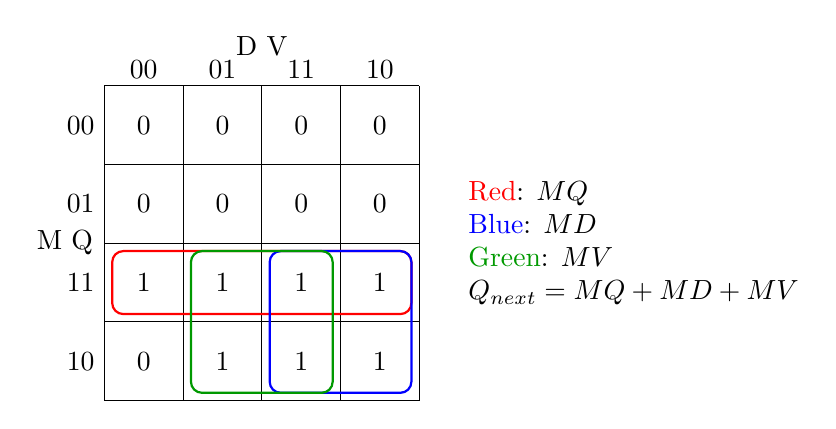
\begin{tikzpicture}
    % Manual K-Map for 4 variables M, D, V, Q
    % We will only draw the relevant map for Q_next
    % Variables: M (MSB), Q, D, V (LSB)? Or M, D, V, Q?
    % Let's use standard map layout.
    % Rows: M Q (00, 01, 11, 10)
    % Cols: D V (00, 01, 11, 10)
    
    \draw (0,0) grid (4,4);
    \node at (2, 4.5) {D V};
    \node at (-0.5, 2) {M Q};
    
    % Column labels
    \node at (0.5, 4.2) {00};
    \node at (1.5, 4.2) {01};
    \node at (2.5, 4.2) {11};
    \node at (3.5, 4.2) {10};
    
    % Row labels
    \node at (-0.3, 3.5) {00};
    \node at (-0.3, 2.5) {01};
    \node at (-0.3, 1.5) {11};
    \node at (-0.3, 0.5) {10};
    
    % Content
    % Q_next = M(Q + D + V)
    % = MQ + MD + MV
    
    % Row 00 (M=0, Q=0): All 0
    \foreach \x in {0.5, 1.5, 2.5, 3.5} \node at (\x, 3.5) {0};
    
    % Row 01 (M=0, Q=1): All 0
    \foreach \x in {0.5, 1.5, 2.5, 3.5} \node at (\x, 2.5) {0};
    
    % Row 11 (M=1, Q=1): All 1 (Because Q=1 makes term MQ=1)
    \foreach \x in {0.5, 1.5, 2.5, 3.5} \node at (\x, 1.5) {1};
    
    % Row 10 (M=1, Q=0): 
    % Need D=1 OR V=1.
    % Cols are D V. 
    % 00 -> 0
    % 01 -> 1
    % 11 -> 1
    % 10 -> 1
    \node at (0.5, 0.5) {0};
    \node at (1.5, 0.5) {1};
    \node at (2.5, 0.5) {1};
    \node at (3.5, 0.5) {1};
    
    % Groups (simplified visual)
    % Group 1: Row 11 (All 1s) -> Term MQ
    \draw[red, rounded corners, thick] (0.1, 1.1) rectangle (3.9, 1.9);
    
    % Group 2: Cols 01, 11, 10 in Row 10 combined with Row 11
    % Actually simpler:
    % Group MQ: Row 11.
    % Group MD: Cols 11, 10 (D=1) in Rows 11, 10 (M=1).
    \draw[blue, rounded corners, thick] (2.1, 0.1) rectangle (3.9, 1.9);
    
    % Group MV: Cols 01, 11 (V=1) in Rows 11, 10 (M=1).
    \draw[green!60!black, rounded corners, thick] (1.1, 0.1) rectangle (2.9, 1.9);

    \node[right, align=left] at (4.5, 2) {
    \textcolor{red}{Red}: $MQ$ \\
    \textcolor{blue}{Blue}: $MD$ \\
    \textcolor{green!60!black}{Green}: $MV$ \\
    \textbf{$Q_{next} = MQ + MD + MV$}
    };

\end{tikzpicture}
\end{document}
